
\section{Neulesuunnittelukilpailu}\label{sec:neulekilpailu}

\begin{wrapfigure}{r}{0.25\textwidth}
	\noindent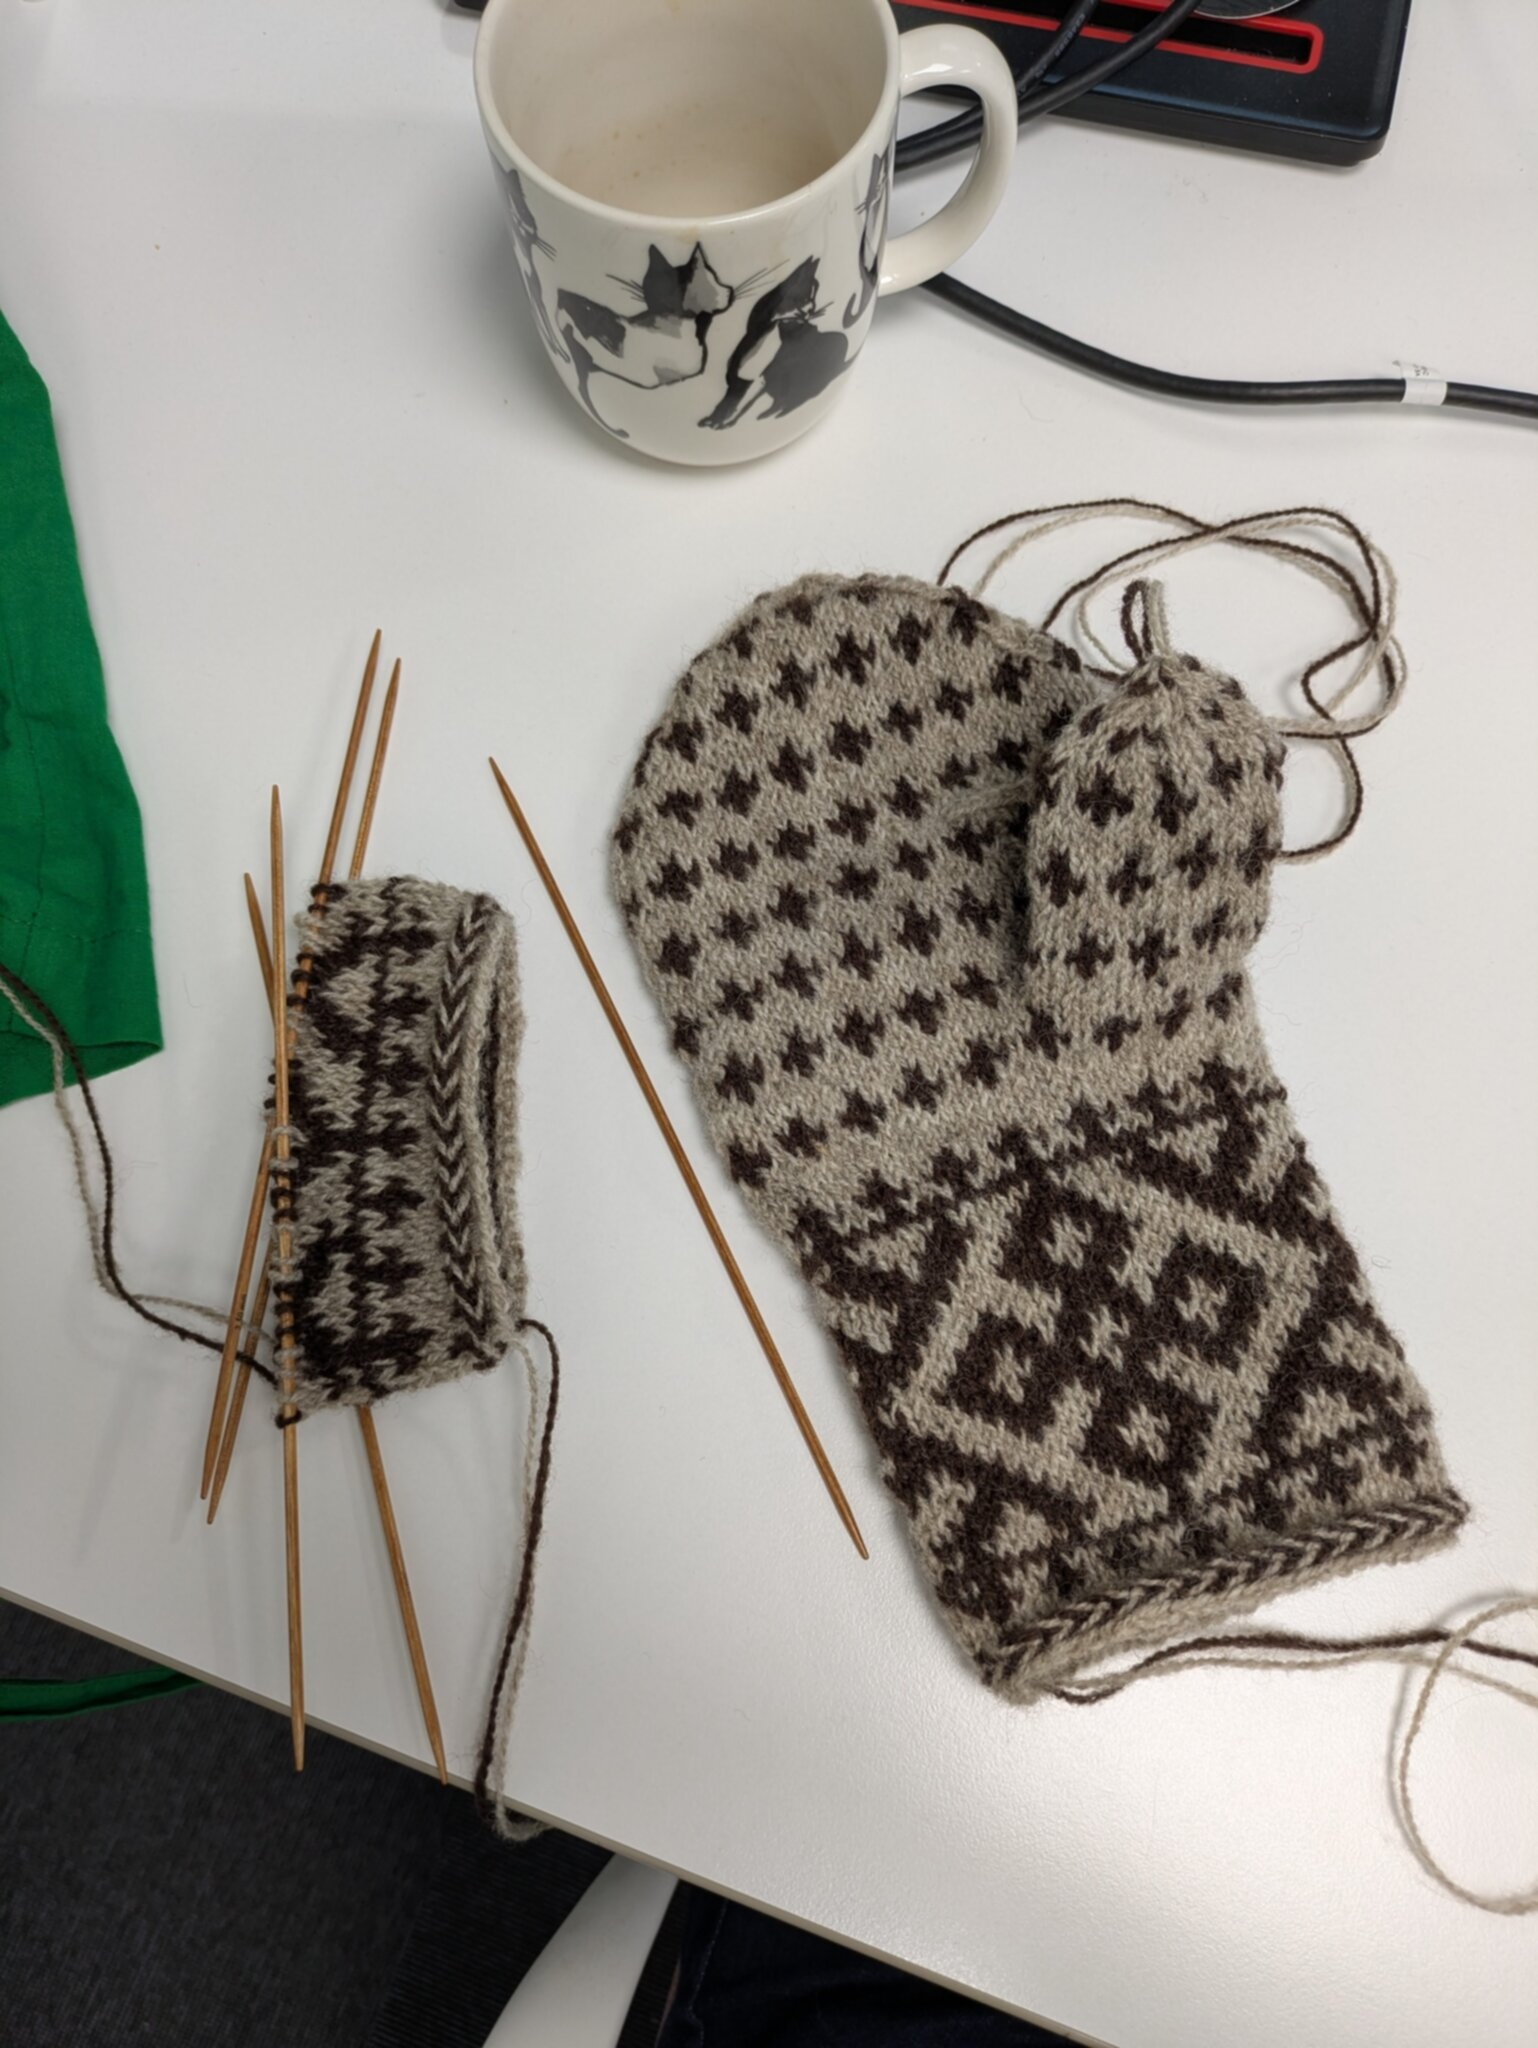
\includegraphics[width=0.9\linewidth]{assets/neulekilpailu1}
\end{wrapfigure}

Osallistumalla tähän Tassun seuraavaan kilpailuun saatat ehkä olla \textbf{se},
joka suunnittelee KuRun seuraavan puolivirallisen vaatekappaleen. Me
ajattelimme, että olisi mukavaa saada KuRun oma neuleohje, jota kaikki
halukkaat jäsenet voisivat neuloa {\tiny(tai voisivat saada jonkun neulomaan
heille\ldots)} ja käyttää ylpeydellä.

Vaikka se näyttää siltä, että järjestämme kilpailun vain Anninalle,
\mbox{Nonnalle} ja Tanguylle, me haluamme että se olisi mahdollisimman avoin
kaikille, myös niille, joilla ei ole ollenkään kokemusta neulesuunnittelusta
eikä neulomisesta. Täysin valmista neulepiirrosta ei tarviste palauttaa, eikä
\mbox{tarkkoja} silmukkalukuja ja kaikkea muuta. Jos sinulla on visio,
piirustuksia tai vain ideoita, kaikki käy, ja voidaan valmistella
täydelliset ohjeet sen jälkeen, kun voittaja on valittu.

Vaatekappalleen tyyppi jätetään osallistujien päätettäväksi, mutta haluamme
että se olisi selläinen, että useimmat voivat toteuttaa sen, olematta
konkareita, esim. lapaset, sukat, pipo, huivi, vaikkapa kypärämyssy!

\bigskip
\noindent Arvostelemme ehdotukset seuraavien kriteerien perusteella:
\vspace{-0.16cm}
\begin{itemize}
\setlength\itemsep{-0.16cm}
\setlength\itemindent{0.64cm}
\item kauneus (hyvin subjektiivista, kyllä kyllä)
\item neulomisen helppous
\item ``KuRulaisuus''
\end{itemize}

\smallskip
Osallistu kilpailuun lähettämällä ehdotuksesi Tassun päätoimittajalle
sähköpostilla (osoitteen löydät lehden sisäkannesta) tai suoraan esimerkiksi
Whatsapp"-viestillä. Julkaisemme voittajan seuraavassa Tassussa.

\vspace{0.32cm}
\begin{center}
	\noindent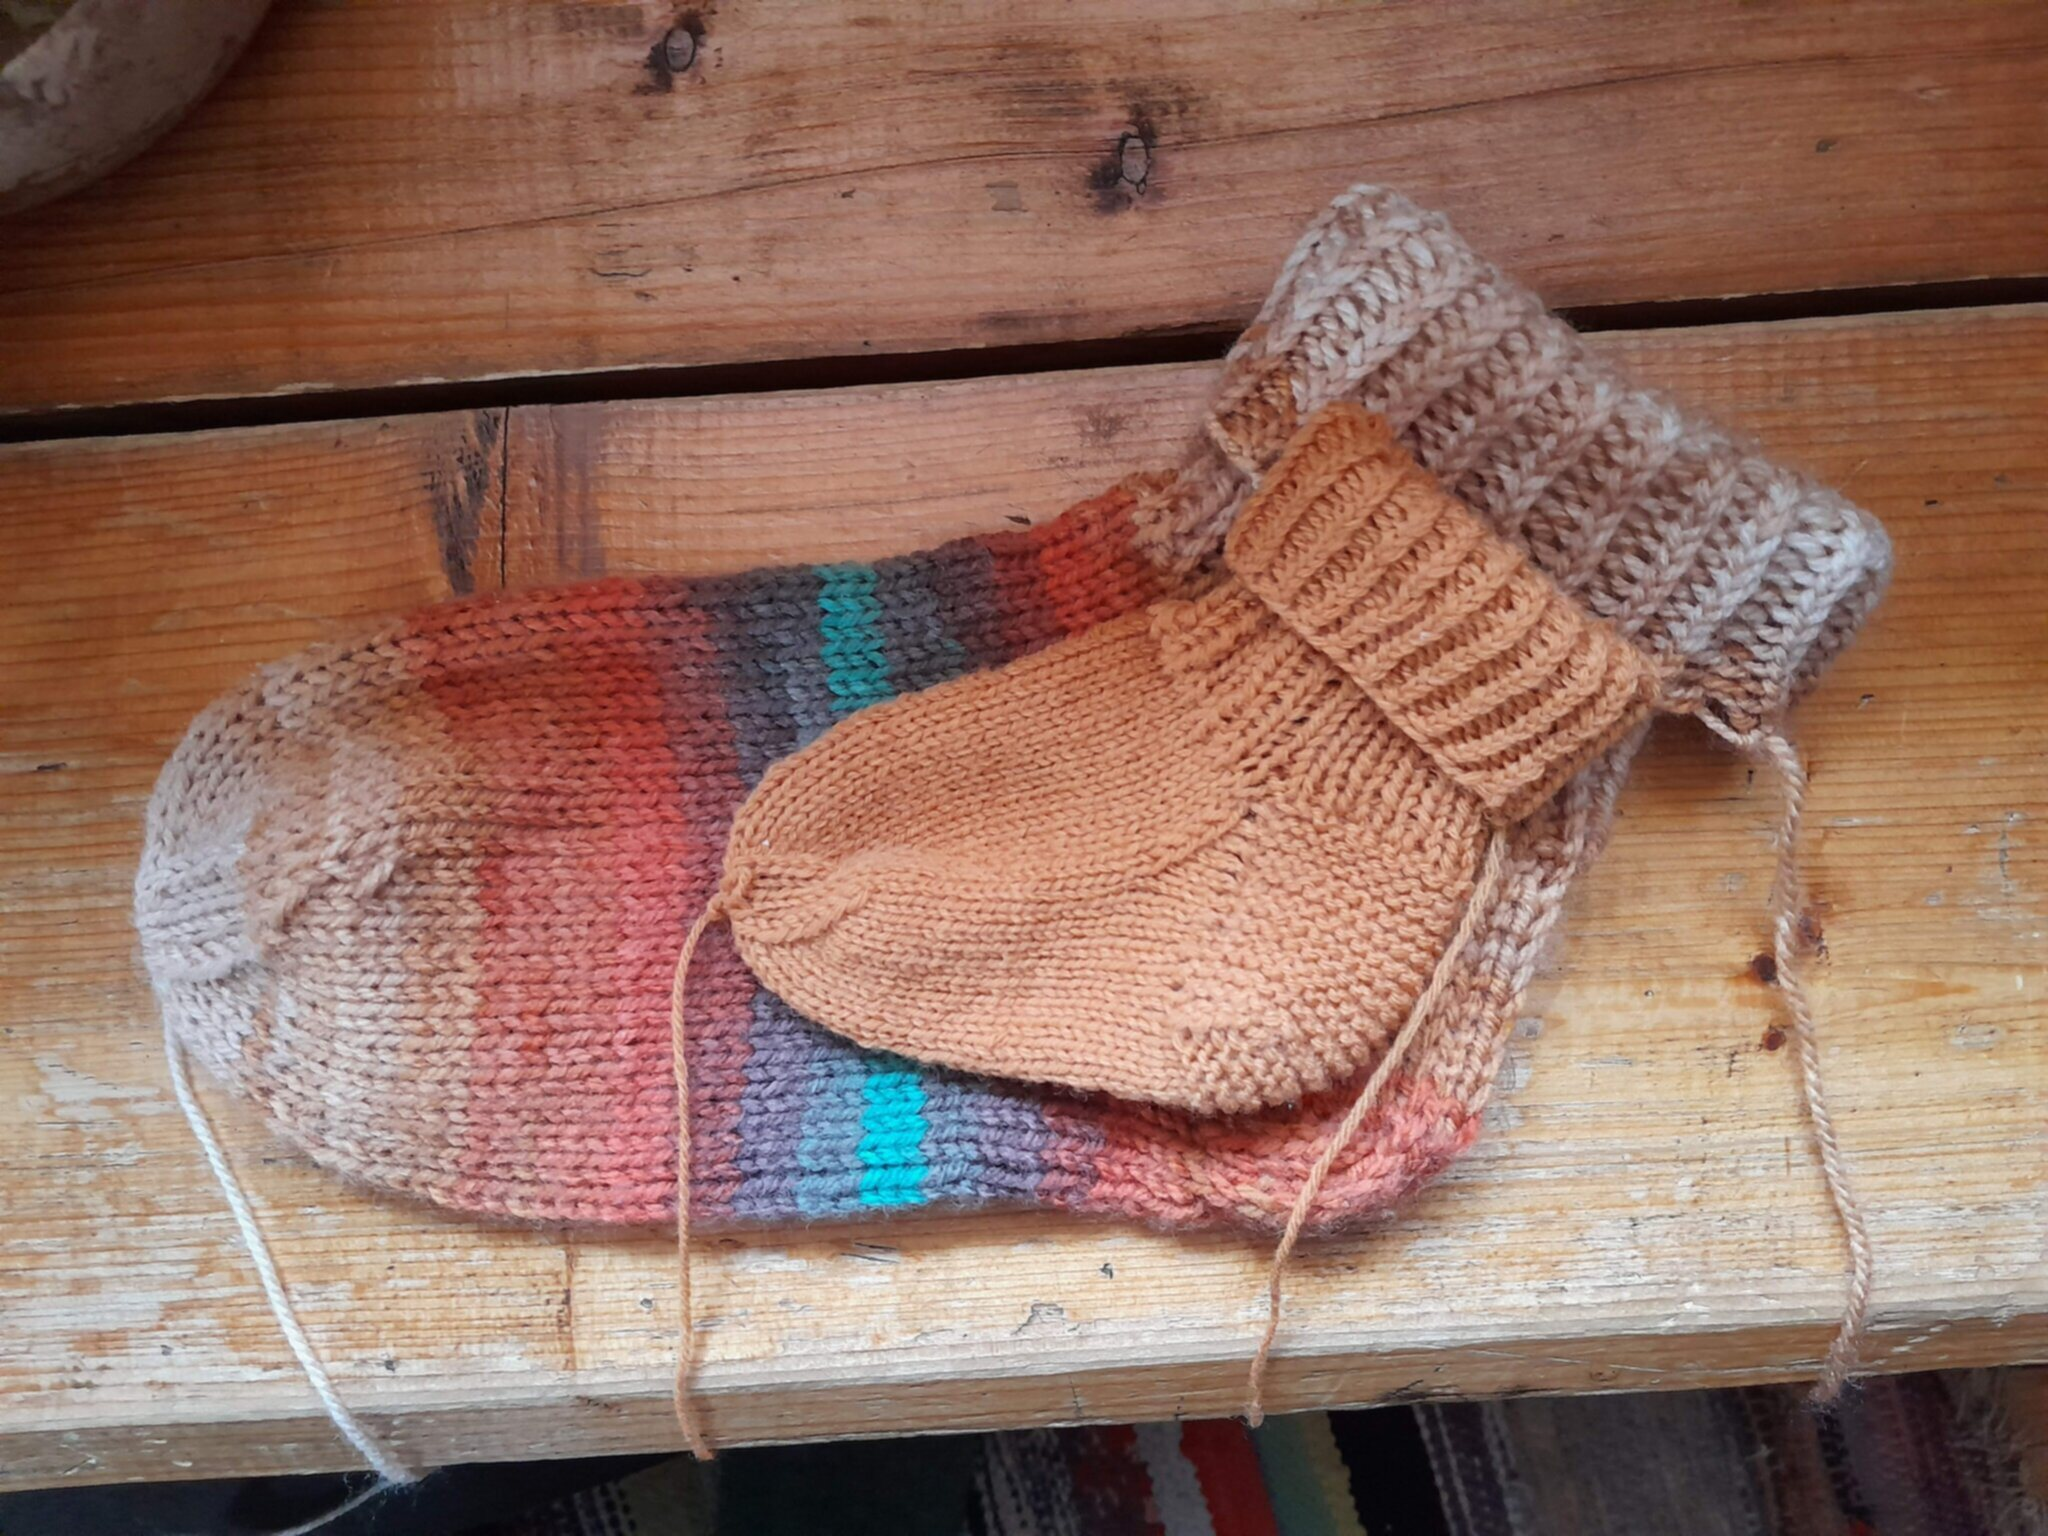
\includegraphics[width=0.8\linewidth,trim={0 9cm 0 9cm},clip]{assets/neulekilpailu2}
\end{center}
